% Template for ISBI paper; to be used with:
%          spconf.sty  - ICASSP/ICIP LaTeX style file, and
%          IEEEbib.bst - IEEE bibliography style file.
% --------------------------------------------------------------------------
\documentclass{article}
\usepackage{spconf,amsmath,graphicx}

\usepackage{enumitem}
\setlist{nosep, leftmargin=14pt}

\usepackage{mwe} % to get dummy images

\title{Equivariant atlas building using UniGradICON}
%
% Single address.
% ---------------
\name{Author(s) Name(s)\thanks{Some author footnote.}}
\address{Author Affiliation(s)}
%
% For example:
% ------------
%\address{School\\
%	Department\\
%	Address}
%
% Two addresses (uncomment and modify for two-address case).
% ----------------------------------------------------------
%\twoauthors
%  {A. Author-one, B. Author-two\sthanks{Some author footnote.}}
%	{School A-B\\
%	Department A-B\\
%	Address A-B}
%  {C. Author-three, D. Author-four\sthanks{The fourth author performed the work
%	while at ...}}
%	{School C-D\\
%	Department C-D\\
%	Address C-D}
%
% More than two addresses
% -----------------------
% \name{Author Name$^{\star \dagger}$ \qquad Author Name$^{\star}$ \qquad Author Name$^{\dagger}$}
%
% \address{$^{\star}$ Affiliation Number One \\
%     $^{\dagger}$}Affiliation Number Two
%
\begin{document}
\maketitle
\begin{abstract}
	Atlas-building is one of the principle uses of image registration. We want to make a general tool for atlas building based on unigradicon, which does image-to-image registration. We build the atlas. We find that we want to factor out the affine component, which can be defined as "make the approach equivariant to affine transforms" so we get out keymorph. We also try just pre-registering with ANTS to get an affine transform, and an instance optimization hack that turns a deformable registration approach into an affine registration approach. One of these ideas will work better than the others, and we will call the one that works best our innovation, and the others comparison methods.
\end{abstract}
\begin{keywords}
One, two, three, four, five
\end{keywords}
\section{Introduction}
\label{sec:intro}

\section{Methods}

Evaluation:

For all approaches, we measure dice of tibial and femoral cartilage through their atlas. For  evaluating the quality of the affine decomposition, we compute deformation fields with and without an extra affine warp, and verify that they are the same.

ANTs:
ANTs is packaged with an atlas building script. We 

\section{Atlas building}

We begin with an average of all images as the atlas, and then cycle:

Warp all images to the atlas

average

warp the atlas by the average transform back to the images

The result is that the expected warp from any pixel in the atlas is zero.

\section{UniGradICON with affine pre-registration}

uniGradICON is a convenient deep registration tool that does not require new training, but it does not provide separate affine and deformable components of the deformation field. We use unigradICON to compute a transform decomposed into an affine and deformable component as follows:

Registration algorithms $\Phi$ (uniGradICON, pretrained) and 

$$\Psi_\theta[I^A, I^B](x) = exp(\theta - \theta^T)[x^T 1]^T$$ (rigid)
$$\Psi_\theta[I^A, I^B](x) = exp(\theta)[x^T 1]^T$$ (deformable)

(note that to begin with, $\Psi_\theta$ does not depend on $I^A and I^B$

Then, we find

$$ \theta = \text{argmin}_\theta \text{LNCC}(I^A \circ \text{TwoStep}\{\Psi_\theta, \Phi\}[I^A, I^B], I^B) $$

This decomposes the transform into affine and deformable components.  


\begin{figure}[htb]

\begin{minipage}[b]{1.0\linewidth}
  \centering
  \centerline{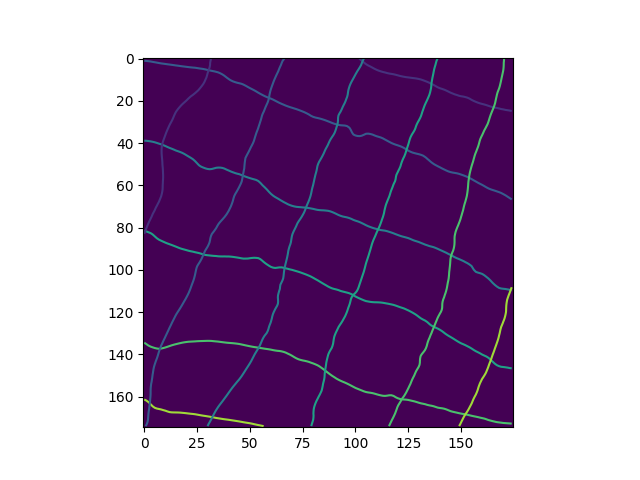
\includegraphics[width=8.5cm]{knee_affine-31/003_.png}}
%  \vspace{2.0cm}
  \centerline{(a) Overall deformation}\medskip
\end{minipage}
%
\begin{minipage}[b]{.48\linewidth}
  \centering
  \centerline{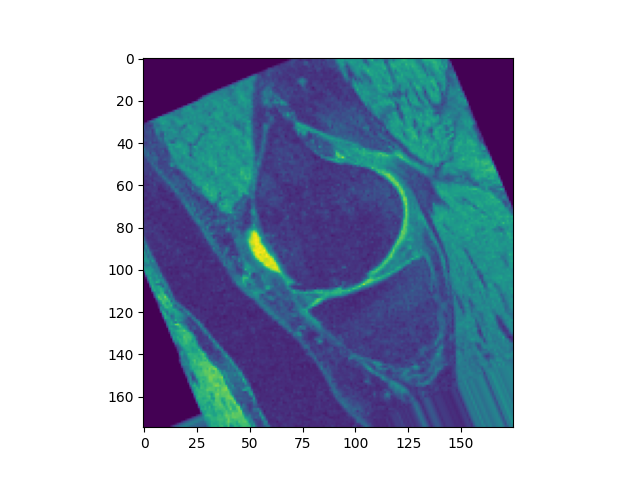
\includegraphics[width=4.0cm]{knee_affine-31/006_.png}}
%  \vspace{1.5cm}
  \centerline{(b) Moving image}\medskip
\end{minipage}
\hfill
\begin{minipage}[b]{0.48\linewidth}
  \centering
  \centerline{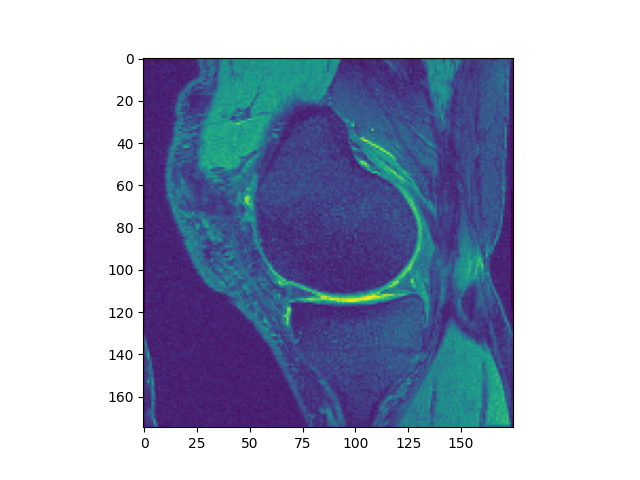
\includegraphics[width=4.0cm]{knee_affine-31/007_.png}}
%  \vspace{1.5cm}
  \centerline{Fixed Image}\medskip
\end{minipage}
%
\begin{minipage}[b]{.48\linewidth}
  \centering
  \centerline{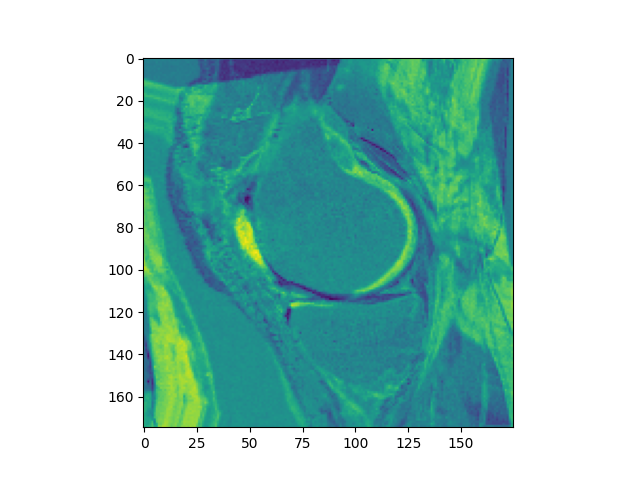
\includegraphics[width=4.0cm]{knee_affine-31/004_.png}}
%  \vspace{1.5cm}
  \centerline{(b) affine alignment}\medskip
\end{minipage}
\hfill
\begin{minipage}[b]{0.48\linewidth}
  \centering
  \centerline{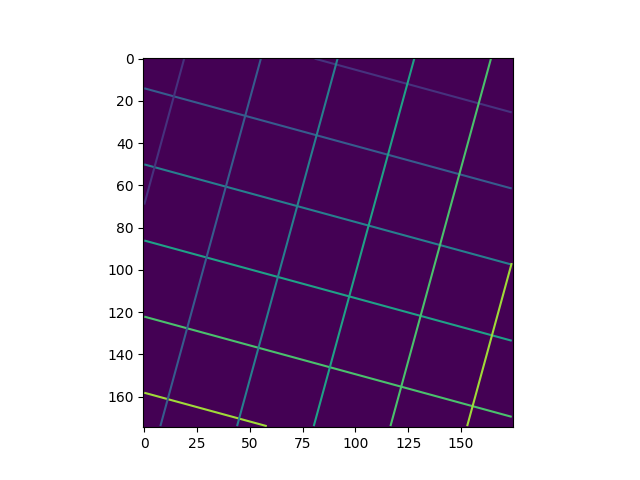
\includegraphics[width=4.0cm]{knee_affine-31/005_.png}}
%  \vspace{1.5cm}
  \centerline{(c) affine component of deformation}\medskip
\end{minipage}
\caption{Example of placing a figure with experimental results.}
\label{fig:res}
%
\end{figure}

% To start a new column (but not a new page) and help balance the last-page
% column length use \vfill\pagebreak.
% -------------------------------------------------------------------------
\vfill
\pagebreak



\section{Compliance with ethical standards}
\label{sec:ethics}

IEEE-ISBI supports the standard requirements on the use of animal and
human subjects for scientific and biomedical research. For all IEEE
ISBI papers reporting data from studies involving human and/or
animal subjects, formal review and approval, or formal review and
waiver, by an appropriate institutional review board or ethics
committee is required and should be stated in the papers. For those
investigators whose Institutions do not have formal ethics review
committees, the principles  outlined in the Helsinki Declaration of
1975, as revised in 2000, should be followed.

Reporting on compliance with ethical standards is required
(irrespective of whether ethical approval was needed for the study) in
the paper. Authors are responsible for correctness of the statements
provided in the manuscript. Examples of appropriate statements
include:
\begin{itemize}
  \item ``This is a numerical simulation study for which no ethical
    approval was required.'' 
  \item ``This research study was conducted retrospectively using
    human subject data made available in open access by (Source
    information). Ethical approval was not required as confirmed by
    the license attached with the open access data.''
    \item ``This study was performed in line with the principles of
      the Declaration of Helsinki. Approval was granted by the Ethics
      Committee of University B (Date.../No. ...).''
\end{itemize}


\bibliographystyle{IEEEbib}
\bibliography{strings,refs}

\end{document}
